\section{Analysis of Interleaver Insertions and Deletions}
Knuth, in Volume 3 of his well-known book \textit{The Art of Computer Programming} \cite{knuth1998art}, mentioned that random insertions and deletions indeed \textit{destroy} the randomness of a BST. Knott\cite{knott1975deletion} and Culberson \& Munro\cite{culberson1990analysis} noticed that, after doing such operations, while the structure of a tree is probabilistically the same, the distribution of keys is not. Eppinger\cite{eppinger1983empirical} demonstrated experimentally that the path length, although initially decreasing slightly, eventually increases and stabilizes after performing a quadratic number of deletions and insertions. Many other articles have also appeared in the literature\cite{jonassen1978trivial, knuth1977deletions}

The following experiment aims to support the observations made by Eppinger and Knuth:
\begin{enumerate}
    \item We create a random BST of size \( n \) by generating \( n \) random keys in the interval \( [0,1] \).
    \item We perform a quadratic number of insertions and deletions as follows: we alternately insert a random element from the interval \( [0,1] \) and delete a random element from the BST.
    \item We compute the internal path length of the BST using a Breadth-First Search algorithm.
    \item We repeat all the previous steps with 20 different seeds and compute the final average.
    \item We repeat the entire experiment for different values of \( n \).
\end{enumerate}

This time, as we are doing a quadratic number of steps, because of memory and time performance I have decided to conduct this experient with Random BSTs of size $1000$ to $2000$ in increases of $50$ elements (same seeds as section \ref{sub:insEx}). Figure \ref{fig:plotDeletion} provides a plot of the final IPL with and without doing this alternation between deletions and insertion. As expected, we see that, indeed, the IPL of a tree increases if we perform this operations, indicating that we are unbalancing our random BST (hence, destroying our randomness).

\begin{figure}[ht]
    \centering
    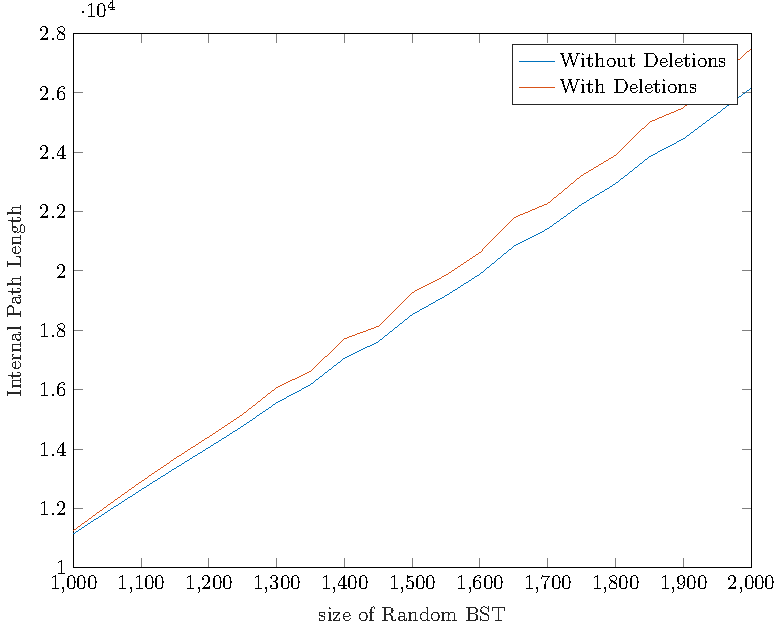
\includegraphics[scale=0.65]{plotDeletion.pdf}
    \caption{Plot average IPL with and without alternating insertions and deletions}
    \label{fig:plotDeletion}
\end{figure}

\newpage

Table \ref{tab:tabDelet} provides a more numerical view of such plot. As we see, the difference in IPL gets bigger as we increases the size of $n$, definitely destroying the initial randomness that we created.

\begin{table}[ht]
    \centering
    \begin{tabular}{|c|c|c|c|}
        \hline 
        $n$ & No Deletions & Deletions & Difference \\ 
        \hline 
        1000 & 11145.85 & 11252.15 & 106.3 \\ 
        1050 & 11890.2 & 12086.95 & 196.75 \\ 
        1100 & 12627.65 & 12900.5 & 272.85 \\ 
        1150 & 13348.65 & 13680.2 & 331.55 \\ 
        1200 & 14053.475 & 14414.25 & 360.775 \\ 
        1250 & 14773.025 & 15172.7 & 399.675 \\ 
        1300 & 15557.95 & 16072.8 & 514.85 \\ 
        1350 & 16171.5 & 16617.6 & 446.1 \\ 
        1400 & 17062.5 & 17715.25 & 652.75 \\ 
        1450 & 17615.975 & 18136.7 & 520.725 \\ 
        1500 & 18530.425 & 19268.7 & 738.275 \\ 
        1550 & 19169.875 & 19860.2 & 690.325 \\ 
        1600 & 19894.3 & 20618.35 & 724.05 \\ 
        1650 & 20830.225 & 21792 & 961.775 \\ 
        1700 & 21419.875 & 22272.1 & 852.225 \\ 
        1750 & 22243.3 & 23213 & 969.7 \\ 
        1800 & 22937.55 & 23899.25 & 961.7 \\ 
        1850 & 23848.45 & 25009.05 & 1160.6 \\ 
        1900 & 24447.525 & 25495.45 & 1047.925 \\ 
        1950 & 25295.475 & 26473.65 & 1178.175 \\ 
        2000 & 26161.125 & 27483.5 & 1322.375 \\ 
        \hline 
    \end{tabular}
    \caption{Difference of IPL after doing deletions}
    \label{tab:tabDelet}
\end{table}


For a more detailed view of Eppinger's work we provide the following experiment:

\begin{enumerate}
    \item We create a random BST of size \( n \) by generating \( n \) random keys in the interval \( [0,1] \).
    \item We perform a quadratic number of insertions and deletions as follows: we alternately insert a random element from the interval \( [0,1] \) and delete a random element from the BST.
    \item We compute the internal path length of the BST using a Breadth-First Search algorithm every $n$ iterations.
    \item We repeat all the previous steps with 20 different seeds and compute the final average.
    \item We repeat the entire experiment for different values of \( n \in \{1000, 1500, 2000\} \).
\end{enumerate}
\newpage

Figure \ref{fig:evIPL} provides a plot of such experiment. Indeed, we see what it was said: The IPL decrease slightly at the beginning but, after that, it starts increasing more than what we had at the beginning. Again, indicating that we are unbalancing our tree and losing our randomness.
\begin{figure}[ht]
    \centering
    \begin{subfigure}{0.32\textwidth}
        \centering
        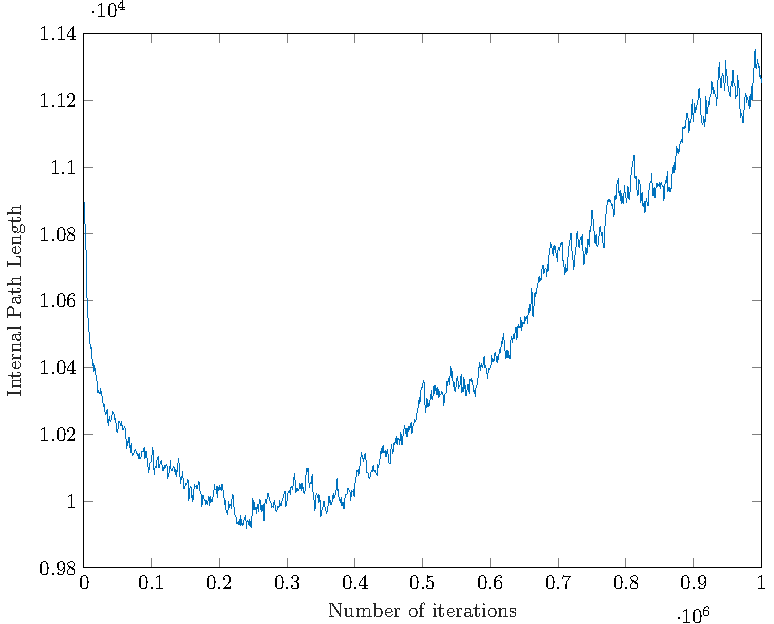
\includegraphics[width=\textwidth]{IPLDelete1000.pdf}
        \caption{Evolution of internal path length by doing insertions and deletions with $n = 1000$}
    \end{subfigure}%
    \hfill
    % Subfigure 2
    \begin{subfigure}{0.32\textwidth}
        \centering
        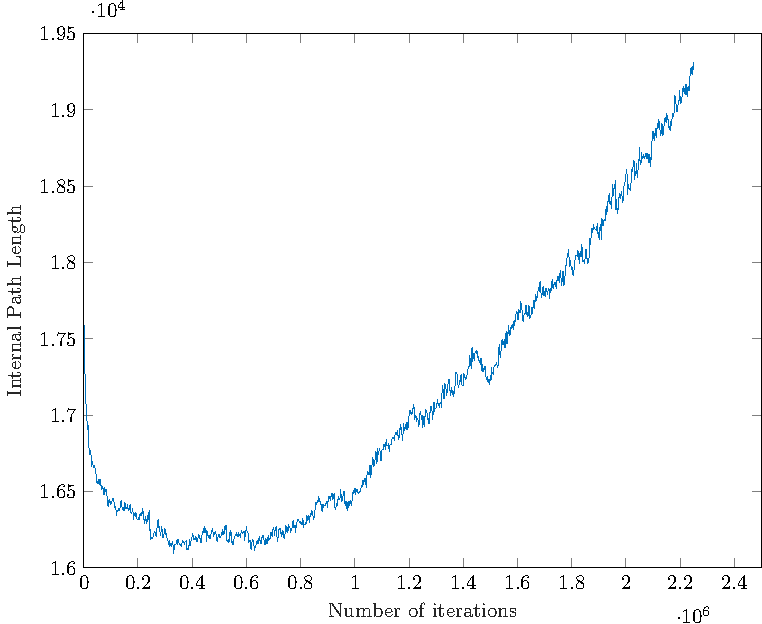
\includegraphics[width=\textwidth]{IPLDelete1500.pdf}
        \caption{Evolution of internal path length by doing insertions and deletions with $n = 1500$}
    \end{subfigure}%
    \hfill
    % Subfigure 3
    \begin{subfigure}{0.32\textwidth}
        \centering
        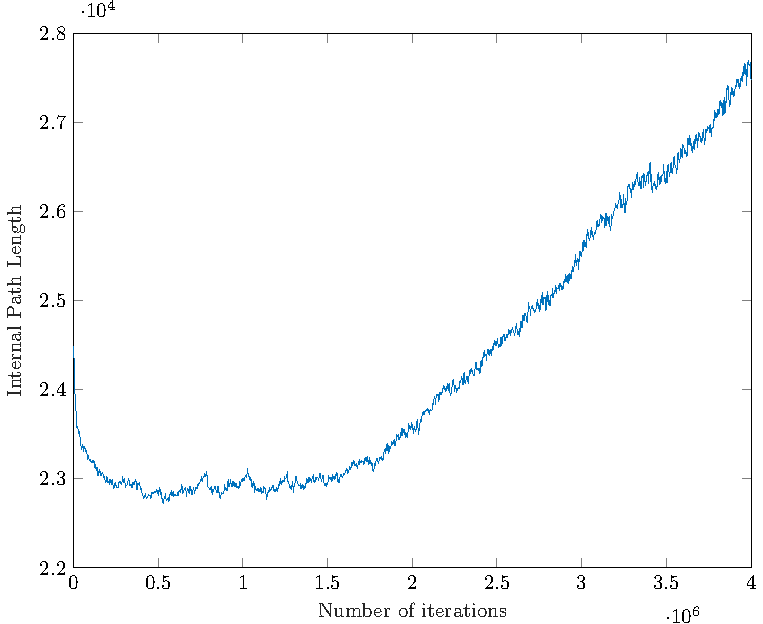
\includegraphics[width=\textwidth]{IPLDelete2000.pdf}
        \caption{Evolution of internal path length by doing insertions and deletions with $n = 2000$}
    \end{subfigure}%
    \caption{Evolution of IPLs by doing insertions and deletions}
    \label{fig:evIPL}
\end{figure}



\section{Conclusion}
Regarding the theoretical analysis of recurrences, although the continuous master theorem is a powerful tool for solving recurrences, it may not always provide a more accurate bound than solving them explicitly.

Regarding the practical part, randomness is a powerful tool for keeping a random BST balanced, but we must be careful in certain situations.

Last but not least, I would like to mention that this last section challenged my intuition: I was expecting that performing random insertions and deletions would not affect the structure of our tree, as every subtree is equally likely.

Special thanks to Conrado's slides on Data Structures and Algorithms, which, along with the book \textit{Introduction to Algorithms}, were a great resource for refreshing my knowledge and assisting me when I struggled with certain calculations!
